\documentclass{scrreprt}

\usepackage{listings}
\usepackage{underscore}
\usepackage{graphicx}
\usepackage[bookmarks=true]{hyperref}
\usepackage[utf8]{inputenc}
\usepackage[portuguese]{babel}
\usepackage{hyperref}
\usepackage{float}

\hypersetup{
	bookmarks=false,    % show bookmarks bar?
	pdftitle={Software Requirement Specification},    % title
	pdfauthor={Grupo 7},                      
	colorlinks=true,       % false: boxed links; true: colored links
	linkcolor=black,       % color of internal links
	citecolor=black,       % color of links to bibliography
	filecolor=black,        % color of file links
	urlcolor=purple,        % color of external links
	linktoc=page            % only page is linked
}
\def\myversion{1.0.3} %Variavel para definir a versao atual
\date{}

\graphicspath{ {./imagens/} }

\begin{document}
	
	\begin{flushright}
		\rule{16cm}{5pt}\vskip1cm
		\begin{bfseries}
			\Huge{SOFTWARE REQUIREMENTS\\ SPECIFICATION}\\
			\vspace{1.cm}
			for\\
			\vspace{1.cm}
			Trash Talker\\
			\vspace{1.cm}
			\LARGE{Version \myversion}\\
			\vspace{1.cm}
			Prepared by:\\ 
			Micael Sampaio (8160202)\\
			João Lopes (8190221)\\
			João Bragança (8190555)\\
			Tiago Leite (8190338)\\
			Flávio Costa (8130247)\\
			\vspace{1.cm}
			Escola Superior de Tecnologia e Gestão \\P.Porto\\
			\vspace{1.cm}
			\today\\
		\end{bfseries}
	\end{flushright}
	
	\tableofcontents
	
	\vspace{4.cm}
	
	\textbf{Histórico de alterações}
	
	
	\begin{tabular}{|p{1.2in}|p{0.7in}|p{2.7in}|p{0.7in}|} \hline 
		\textbf{Nome} & \textbf{Data} & \textbf{Motivo da alteração} & \textbf{Versão} \\ \hline 
		Flávio Costa & 29/10/2021 & Levantamento de requisitos da admnistração & 1.0.0 \\ \hline 
		Tiago Leite & 29/10/2021 & Levantamento de requisitos dos funcionários & 1.0.1 \\ \hline
		Micael Lobo & 08/11/2021 & Use Cases e Âmbito do Produto & 1.0.2 \\ \hline
		João Bragança & 11/11/2021 & Interfaces de Utilizador e Funções do Produto & 1.0.3 \\ \hline 
		Flávio Costa & 08/12/2021 & Revisão dos requisitos e Diagrama de classes & 1.0.4 \\ \hline 
		João Lopes & 22/12/2021 & Revisão dos requisitos e Diagrama de classes & 1.0.5 \\ \hline 	
		Flávio Costa & 10/01/2022 & Revisão dos requisitos e Diagrama de classes & 1.0.6 \\ \hline 
		
	\end{tabular}
	
	
	\chapter{Introdução}
	
	\section{Propósito}
	
	Este documento faz parte da especificação de requisitos de software. Destina-se a registar os requisitos que devem ser incorporados ao sistema a ser construído. Este documento 
	será usado pela equipa de desenvolvimento e por possíveis interessados na sua utilização.
	Os requisitos descritos neste documento específico serão a base para o design e 
	desenvolvimento subsequente de um software capaz de auxiliar empresas de recolha de resíduos para permitir um rigoroso controlo das recolhas,  maximizar a produtividade e automatizar processos.
	
	
	\begin{figure}[H]
		\centering
		
\includegraphics[scale=.90]{imagens/Trash Talker copy.pdf}
		\par Logotipo
		\label{fig:Logotipo}
	\end{figure}
	
	\newpage
	
	\section{Sugestões de Audiência e Leitura Previstas}
	Este documento destina-se a todos os elementos da equipa \textit{SCRUM},
	sendo que existirá três tipos de leitores.
	Sugestão de leitura:
	\begin{itemize}
		\item Product Owner;
		\begin{enumerate}
			\item Propósito;
			\item Âmbito do Produto;
			\item Perspetiva do Produto;
			\item Funções do Produto.
		\end{enumerate}
		\item Scrum Master;
		\begin{enumerate}
			\item Propósito;
			\item Âmbito do Produto;
			\item Perspetiva do Produto;
			\item Funções do Produto.
		\end{enumerate}
		\item Development Team.
		\begin{enumerate}
			\item Propósito;
			\item Perspetiva do Produto;
			\item Requisitos de Interface Externa;
			\item Use Cases.
		\end{enumerate}
	\end{itemize}
	
	
	
	\section{Âmbito do Produto}
	Como foi referido anteriormente, o âmbito deste produto será auxiliar as empresas de recolha de resíduos com o objetivo de facilitar os processos de recolha. Isto é, implementar sensores de distanciamento nos ecopontos permitindo assim saber em tempo real o estado (volume) destes mesmos. Efetivamente, com estes valores é possível programar e configurar rotas conforme o volume desejado dos contentores, otimizando assim os trajetos das recolhas realizadas pela empresa. 

	
	{\let\clearpage\relax \chapter{Descrição Global}}
	
	\section{Perspetiva do Produto}
	\begin{figure}[H]
		\centering
		\includegraphics[scale=.45]{imagens/projectArchitecture}
		\par Project Architecture
		\label{fig:porjectArchitecture}
	\end{figure}
	
	\newpage
	
	\section{Funções do Produto}
	
	Com base nos diferentes tipos de perfil de utilizador o produto final apresenta as seguintes funcionalidades:\newline\newline
	
	\textbf{Administrador}
	\begin{itemize}
		\item Gestão de Manager:
		\begin{itemize}
			\item Criação de perfil de Manager;
		\end{itemize}
	\end{itemize}	
	\textbf{Gestor}
	\begin{itemize}
		\item Gestão de funcionários:
		\begin{itemize}
			\item Criação de perfil do funcionário;
			\item Visualização do perfil do funcionário;
			\item Edição do perfil do funcionário;
			\item Desativar perfil do funcionário.
		\end{itemize}
		\item Gestão de Ecopontos/Contentores:
		\begin{itemize}
			\item Criar ecoponto e associar os respetivos contentores;
			\item Alterar informação do ecoponto e os respetivos contentores;
			\item Desativar ecoponto (caso deixe de exister).
		\end{itemize}
		\item Gerir rotas:
		\begin{itemize}
			\item Criação de rota;
			\item Alteração de rota;
			\item Visualizar rotas;
			\item Desativar rota.
		\end{itemize}
		\item Otimizar rotas:
		\begin{itemize}
			\item Conforme percentagem de ocupação;
			\item Por distância.
		\end{itemize}
		\item Obter dados estatísticos das recolhas:
		\begin{itemize}
			\item Por rota;
			\item Por data(s).
		\end{itemize}
		\item Gerir alertas do sitema:
		\begin{itemize}
			\item Submeter problema;
			\item Visualizar Alertas por Resolver;
			\item Concluir um problema por resolver;
		\end{itemize}
	\end{itemize}
	
	\textbf{Funcionário}
	\begin{itemize}
		\item Iniciar uma Rota;
		\item Registar recolha de um contentor;
		\item Finalizar uma Rota;
		\item Reportar problema.
	\end{itemize}
	
	\begin{figure}[H]
		\centering
		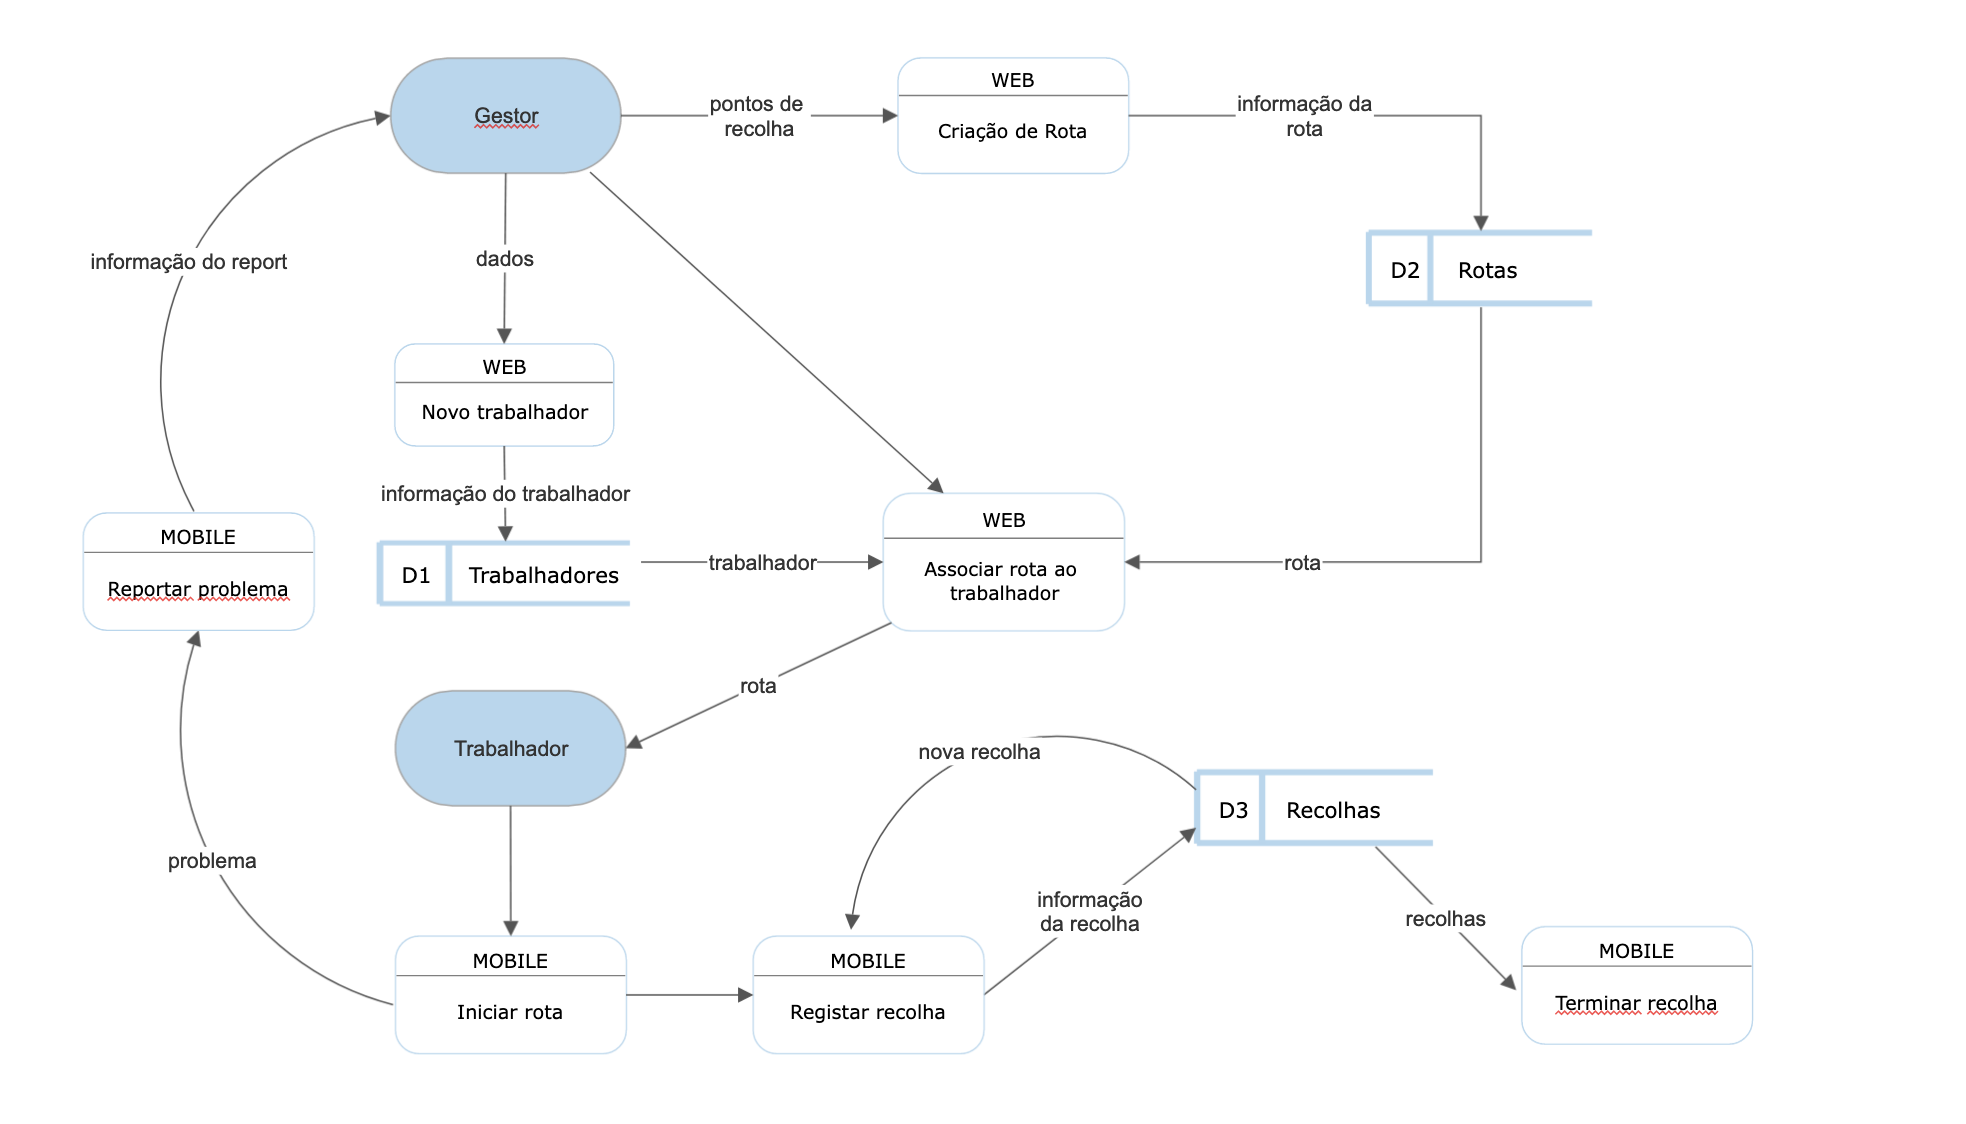
\includegraphics[scale=.55]{imagens/DataFlowDiagram}
		\par \textbf{Data Flow Diagram}
		\label{fig:DataFlowDiagram}
	\end{figure}
	
	\newpage
	
	\section{Classes e Características do Utilizador}
	Essencialmente existirão dois tipos de utilizadores a interagir com o produto, o Gestor que fará o papel de administrador, isto é, que é responsável por gerir/controlar o negócio e os funcionários que irão fazer as recolhas. 
	
	\begin{figure}[H]
		\centering
		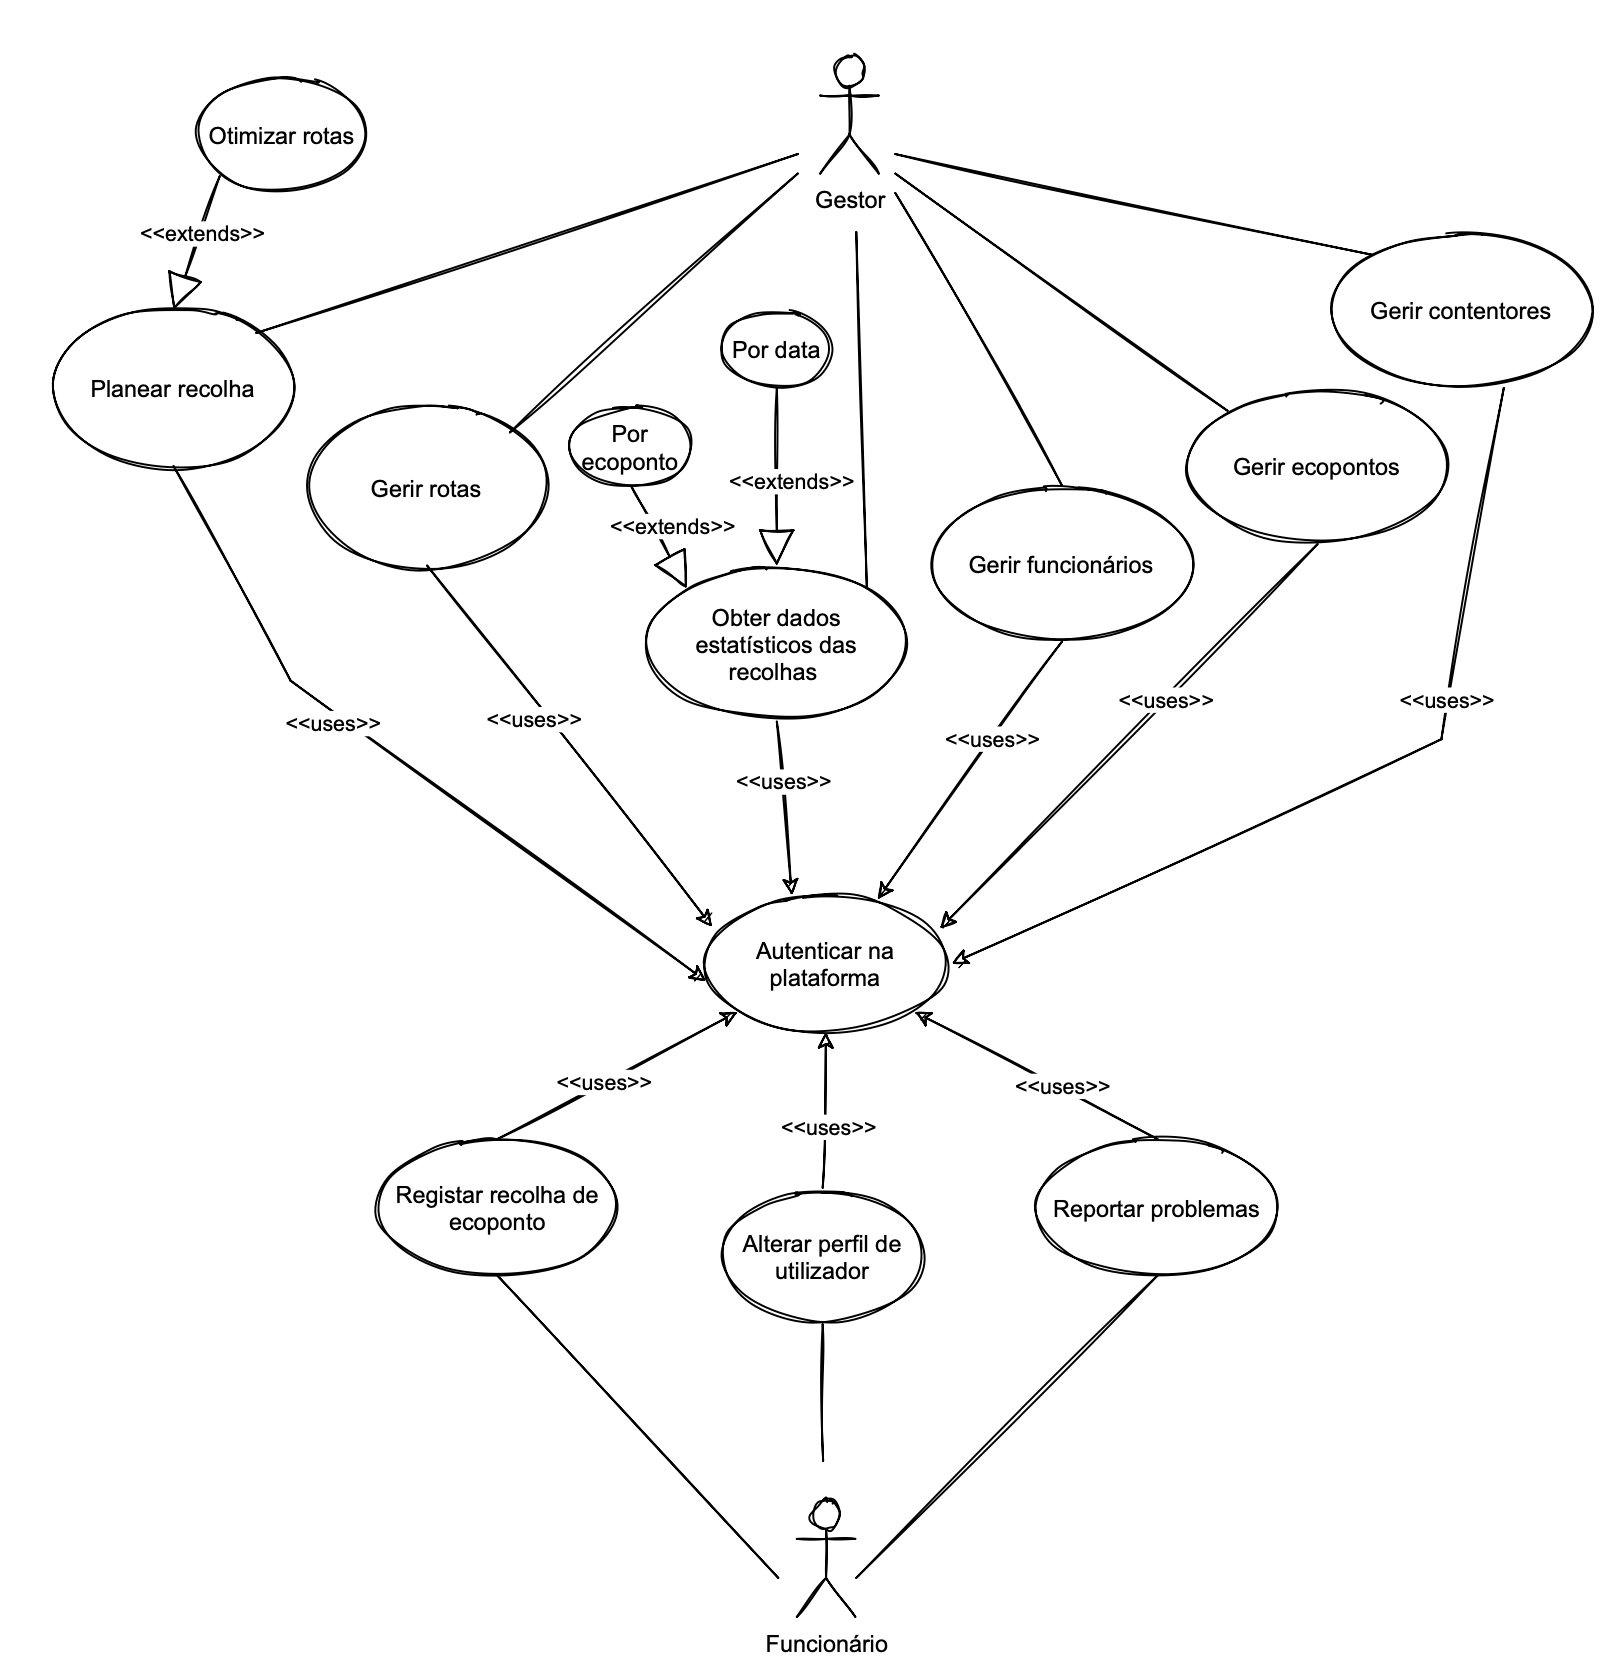
\includegraphics[scale=.60]{imagens/UseCase3}
		\par \textbf{Use Case}
		\label{fig:UseCase3}
	\end{figure}
	
	\newpage
	
	\section{Ambiente Operacional}
	Este produto irá operar essencialmente em duas plataformas.
	A plataforma WEB (Web API) que será utilizada num browser com um devido sistema operativo (windows, linux ou macOS) e será exclusivamente direcionada para o gestor e as suas atividades. Já a plataforma MOBILE que executará num sistema android, terá o objetivo de auxiliar os funcionários na execução das rotas e ser capaz de registar as recolhas efetuadas.
	
	\begin{itemize}
		\item Metodologia SCRUM
		\item Servidor/Backend:
		\begin{itemize}
			\item API: .NET framework, linguagem C\# 
			\item API: .NET framework, linguagem C\# 
			\item Base De Dados: SQL Express
		\end{itemize}
		\item Client/Frontend: 
		\begin{itemize}
			\item Website: Angular
			\item Mobile App: Android, linguagem Kotlin
		\end{itemize}
	\end{itemize}
	
	\section{Pressupostos e Dependências}
	Para o correto funcionamento do produto são necessárias as seguintes dependências:
	\textbf{\large Google API}
	\begin{itemize}
		\item \textbf{Distance Matrix API} - Calcular distâncias entre os diversos locais (matriz de distância).
		\item \textbf{Geocoding API} - Converter moradas em coordenadas geográficas
		\item \textbf{Arduino IoT Cloud} - Comunicação entre o arduino e a cloud
		\item (Outros)
	\end{itemize}
	
	{\let\clearpage\relax \chapter{Requisitos de interface externa}}
	
	\section{Interfaces de Utilizador}
	
	\begin{Large}
		\begin{center}
			\textbf{WEB}
		\end{center}
	\end{Large}

	\begin{figure}[H]
		\centering
		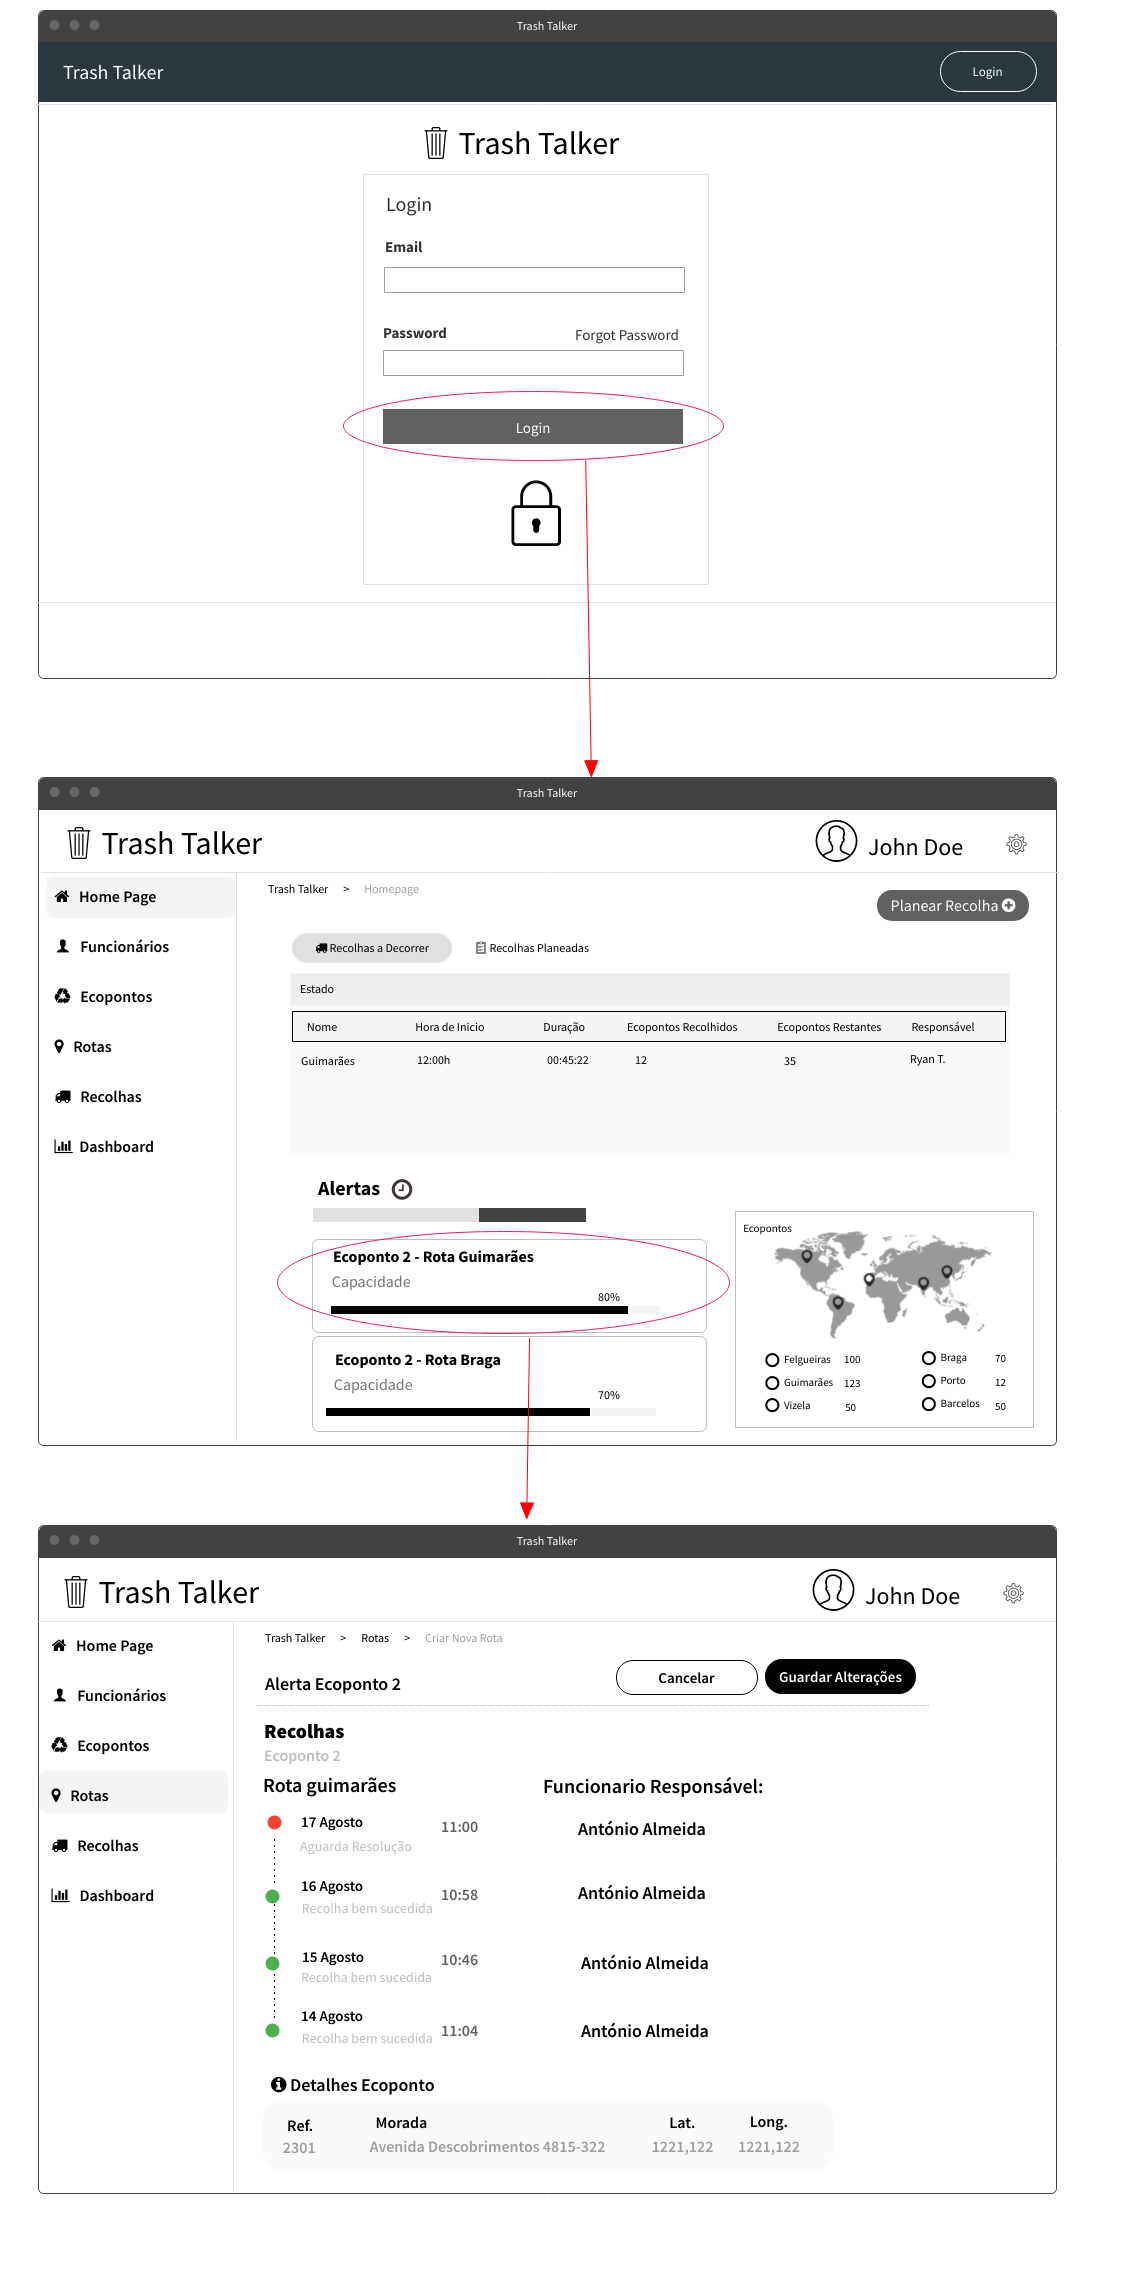
\includegraphics[scale=.30]{imagens/MockupHomepage}
		\par \textbf{Mockup Home Page}
		\label{fig:MockupHomepage}
	\end{figure}
	\begin{figure}[H]
		\centering
		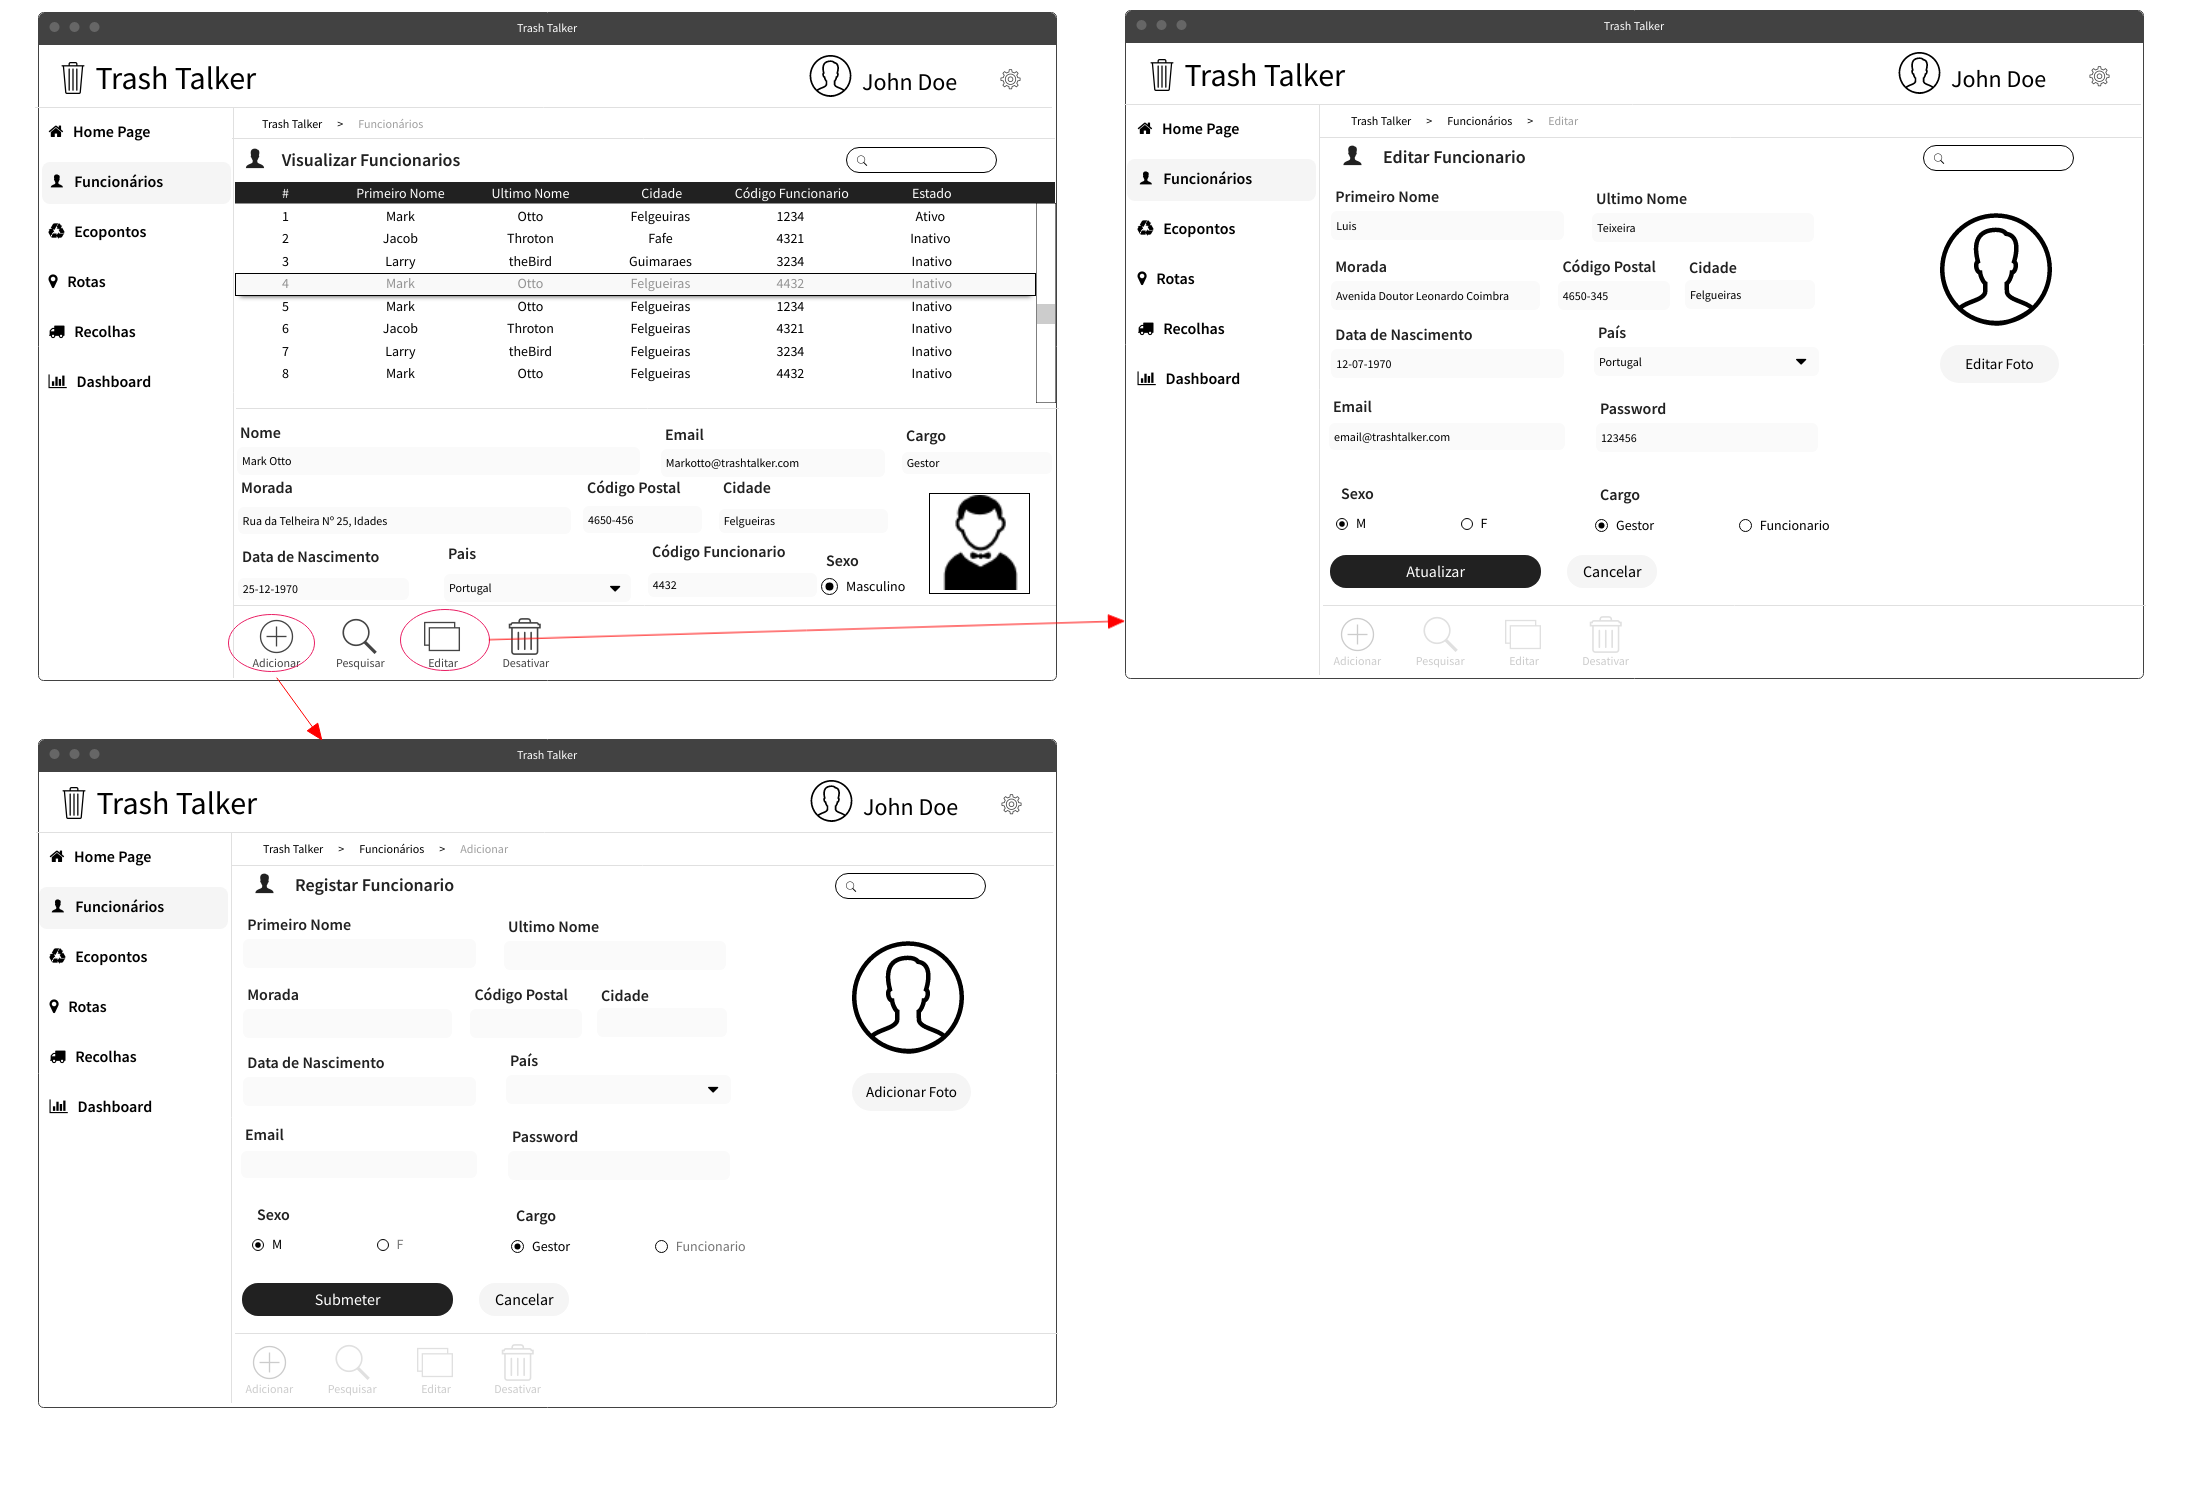
\includegraphics[scale=.23]{imagens/MockupFuncionarios}
		\par \textbf{Mockup Gestão de Funcionários}
		\label{fig:MockupFuncionarios}
	\end{figure}
	\begin{figure}[H]
		\centering
		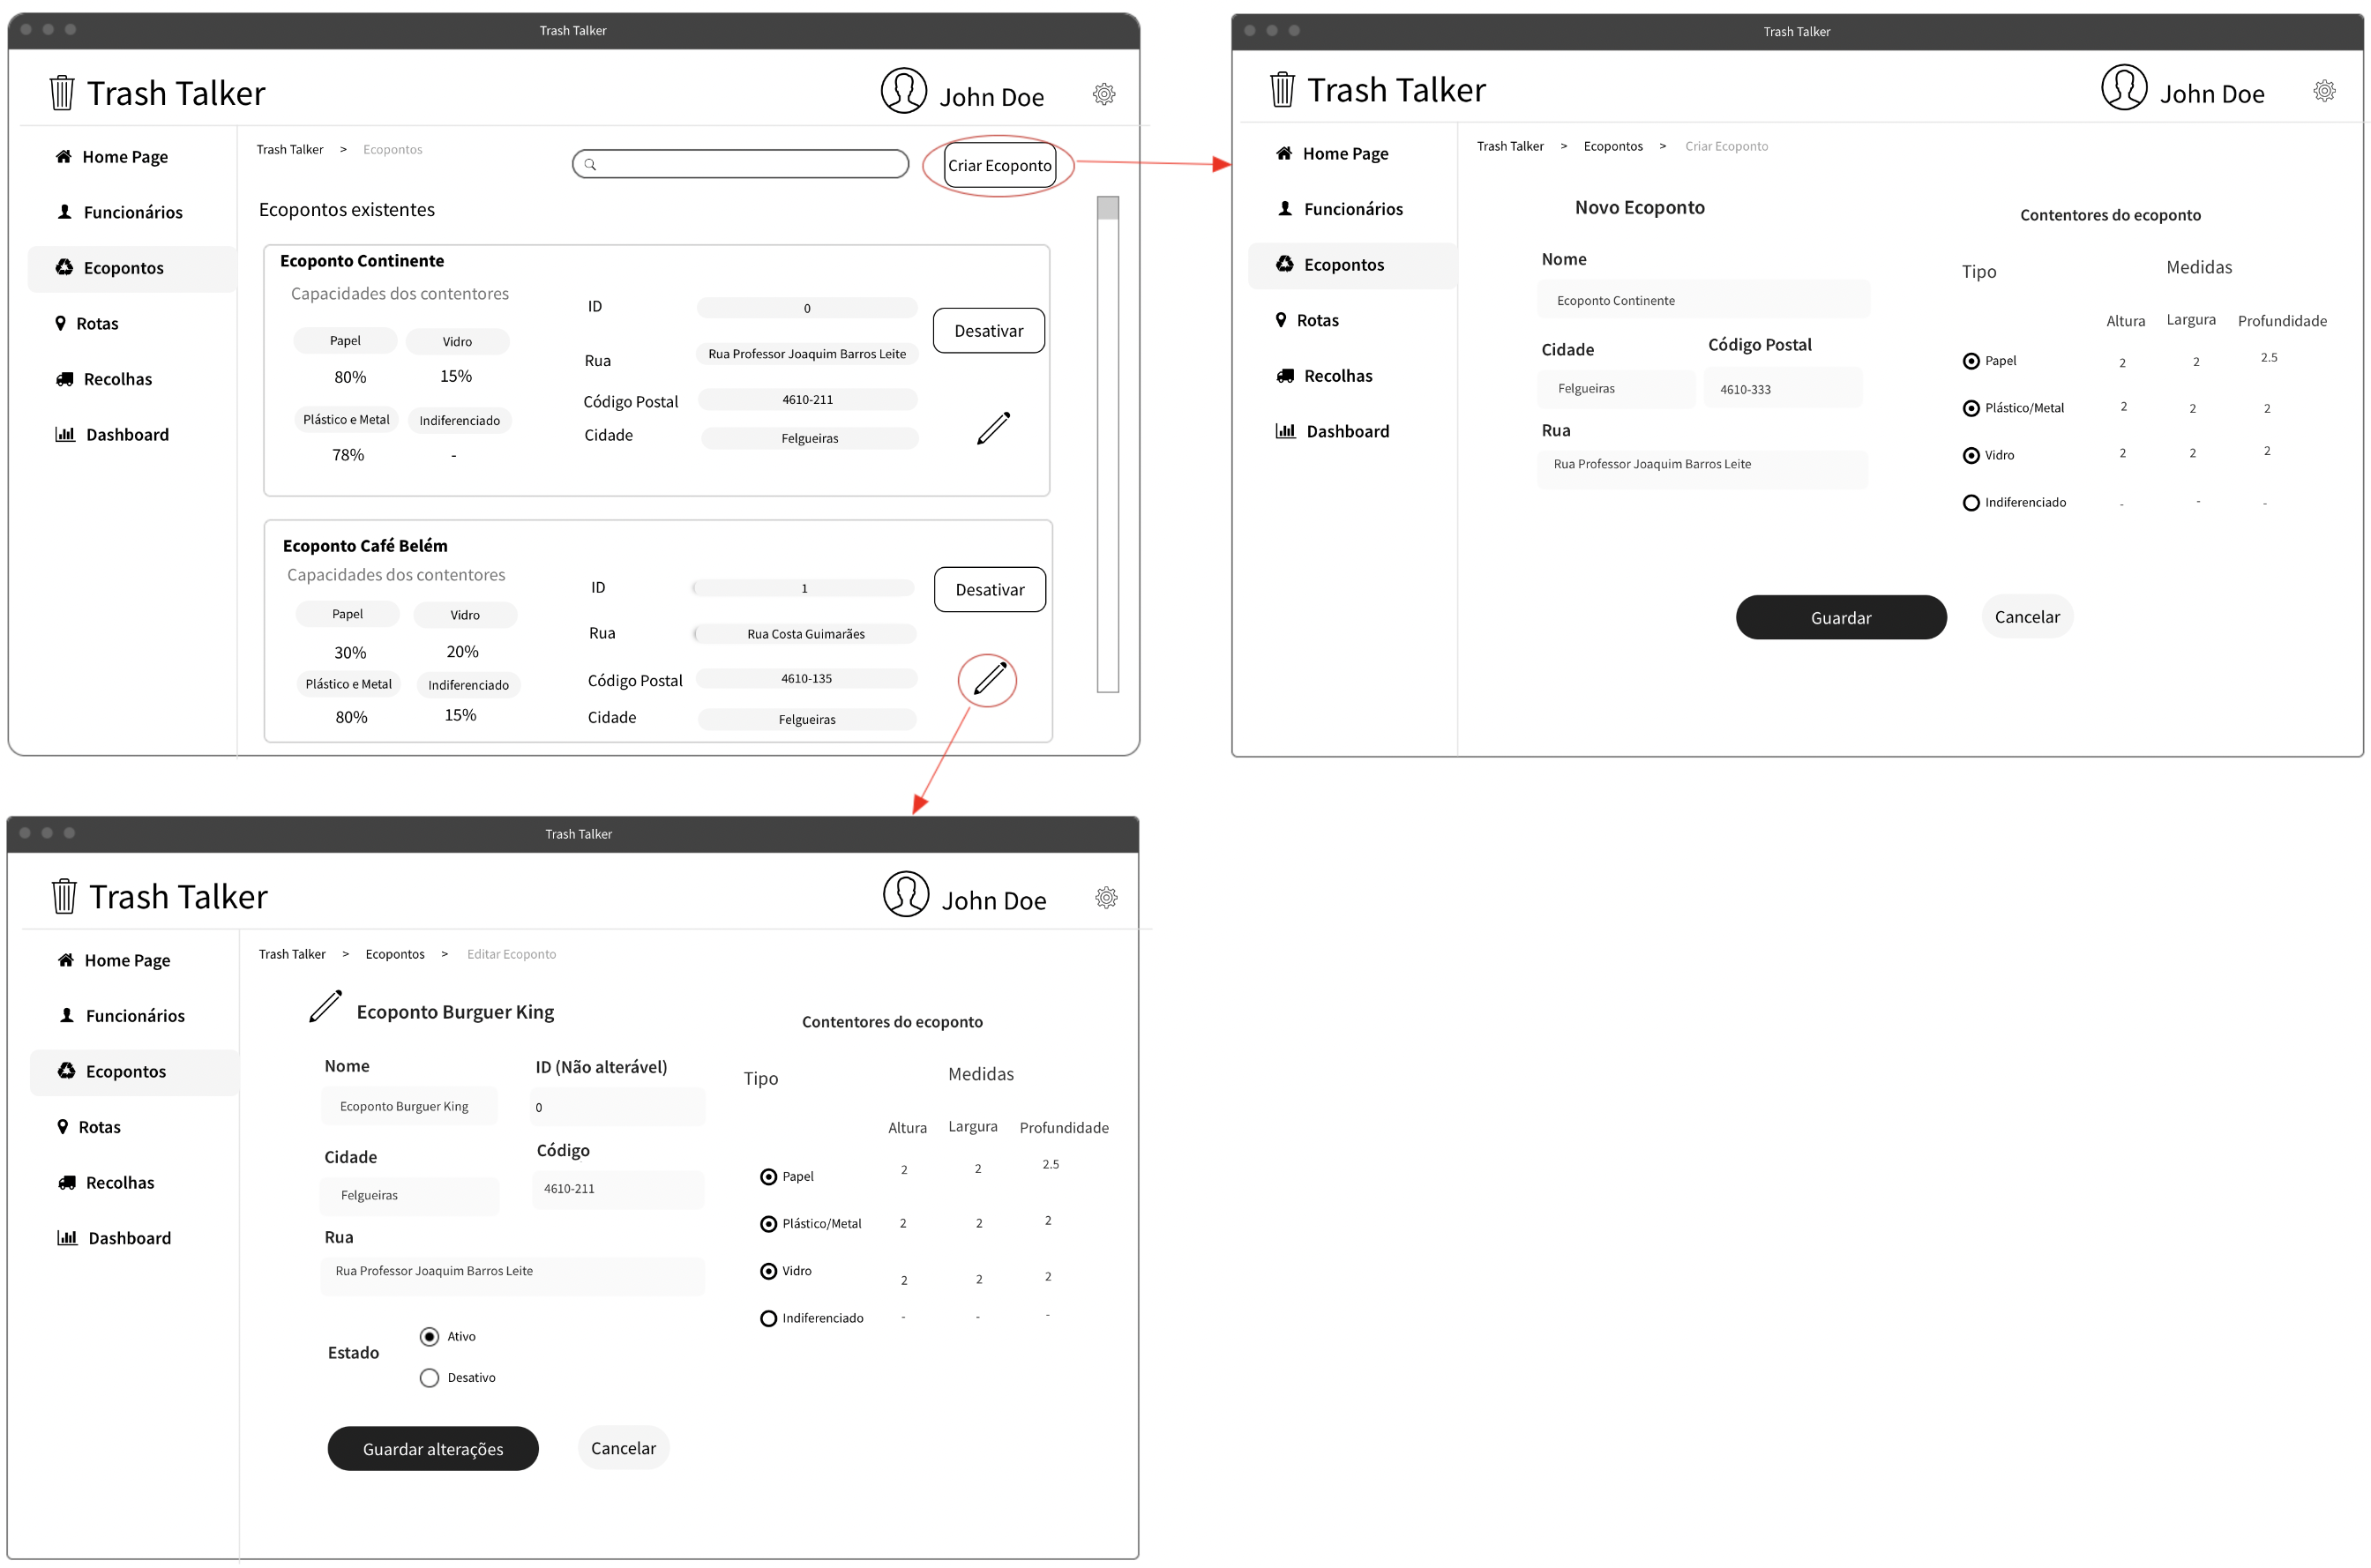
\includegraphics[scale=.36]{imagens/MockupEcopontos}
		\par \textbf{Mockup Gestão de Ecopontos}
		\label{fig:MockupEcopontos}
	\end{figure}
	\newpage
	\begin{figure}[H]
		\centering
		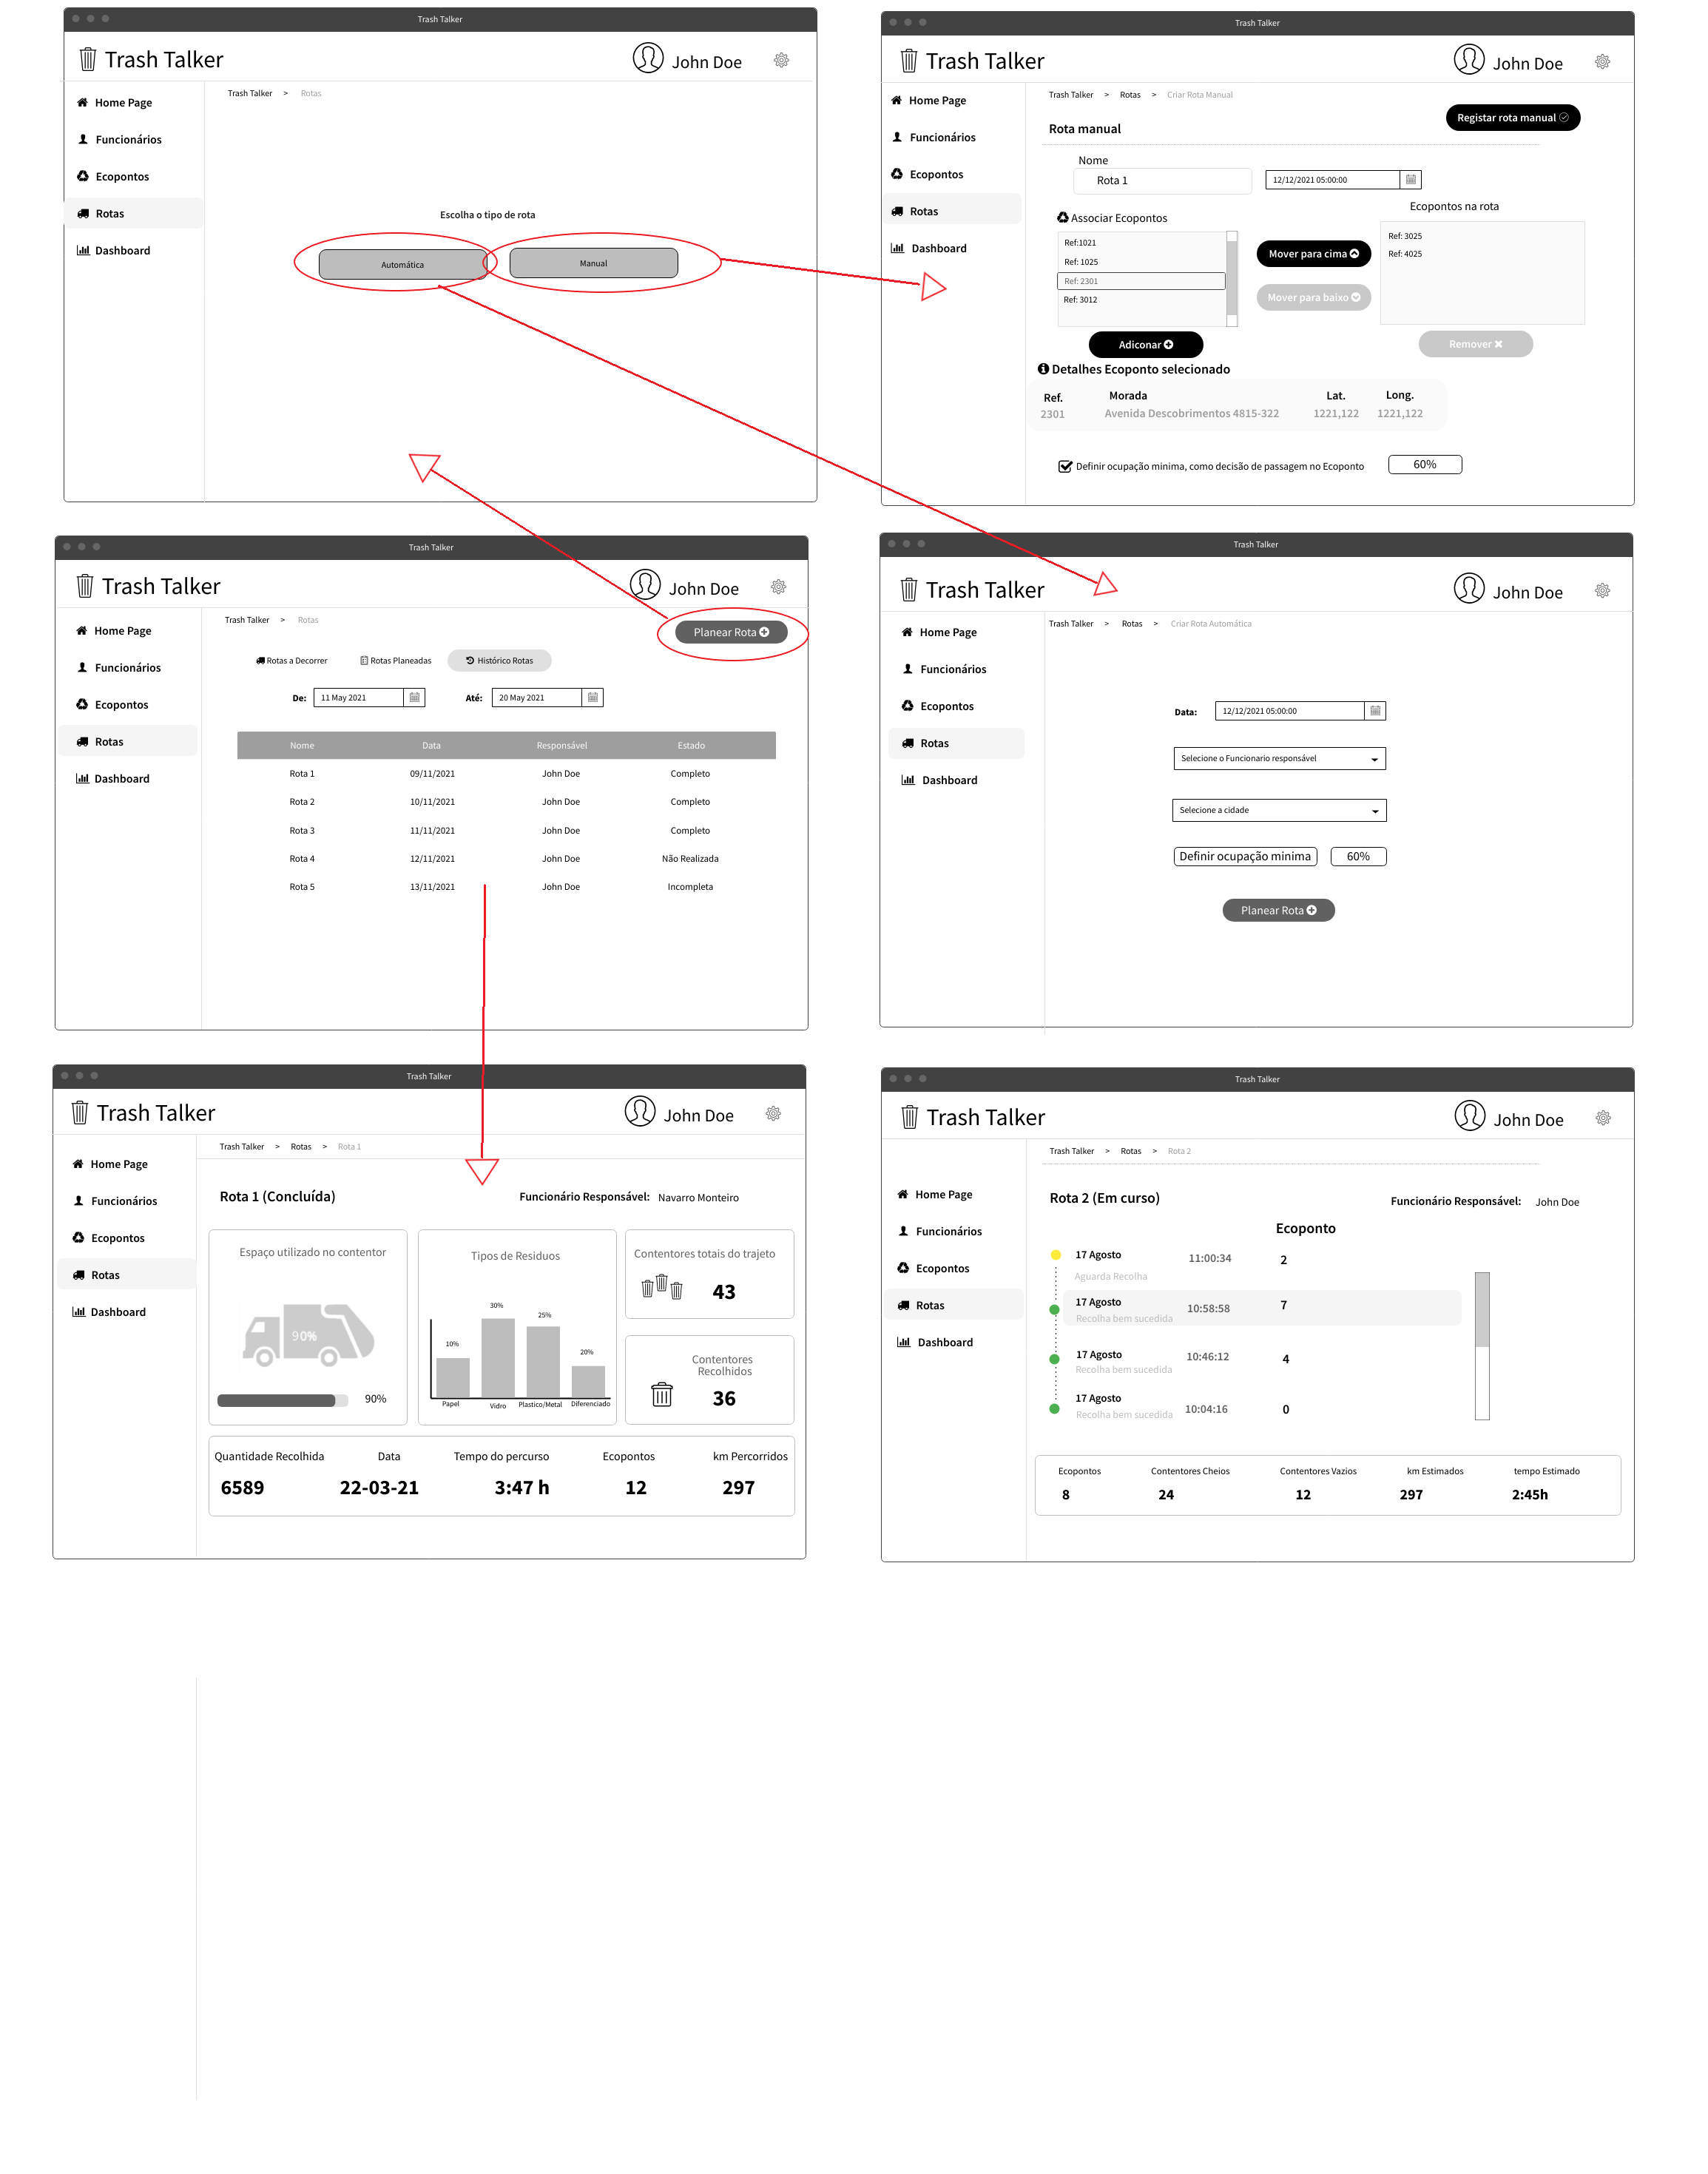
\includegraphics[scale=.27]{imagens/MockupRotas}
		\par \textbf{Mockup Gestão de Rotas}
		\label{fig:MockupRotas}
	\end{figure}
	
	\begin{figure}[H]
		\centering
		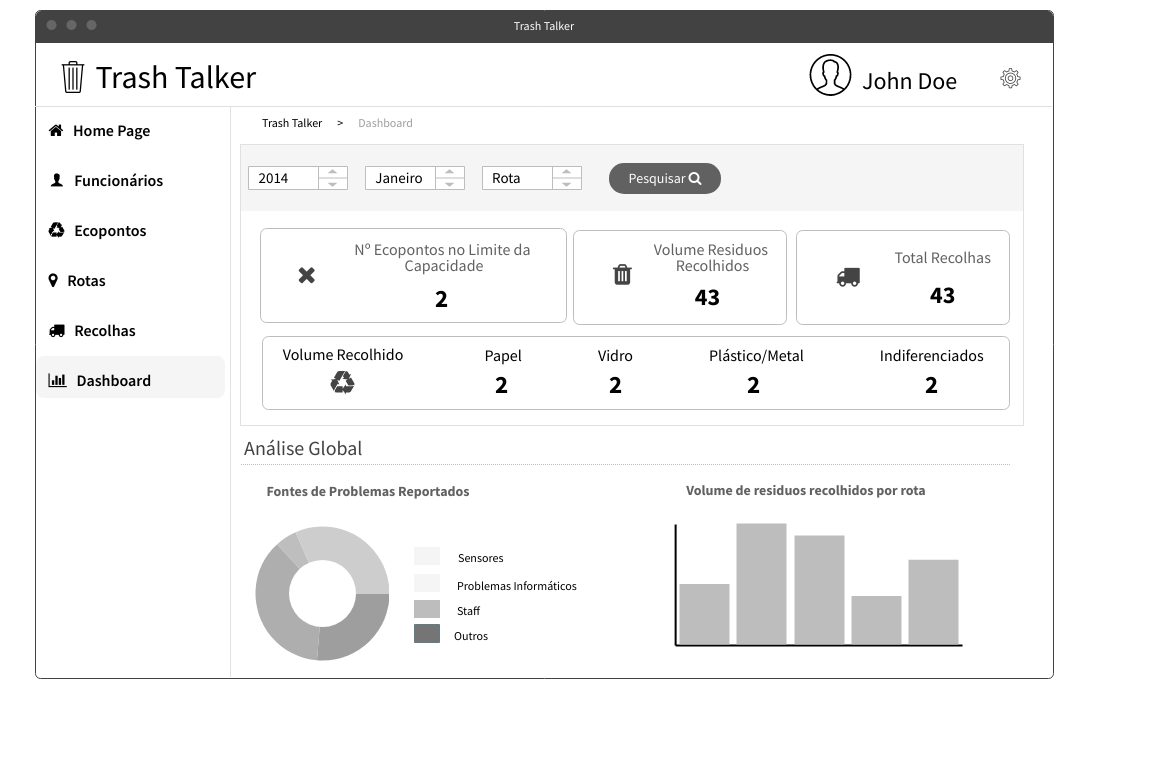
\includegraphics[scale=.40]{imagens/MockupDashboard}
		\par \textbf{Mockup Dashboard}
		\label{fig:MockupDashboard}
	\end{figure}
	
	\newpage
	\begin{Large}
		\begin{center}
			\textbf{MOBILE}
		\end{center}
	\end{Large}
	
	\begin{figure}[H]
		\centering
		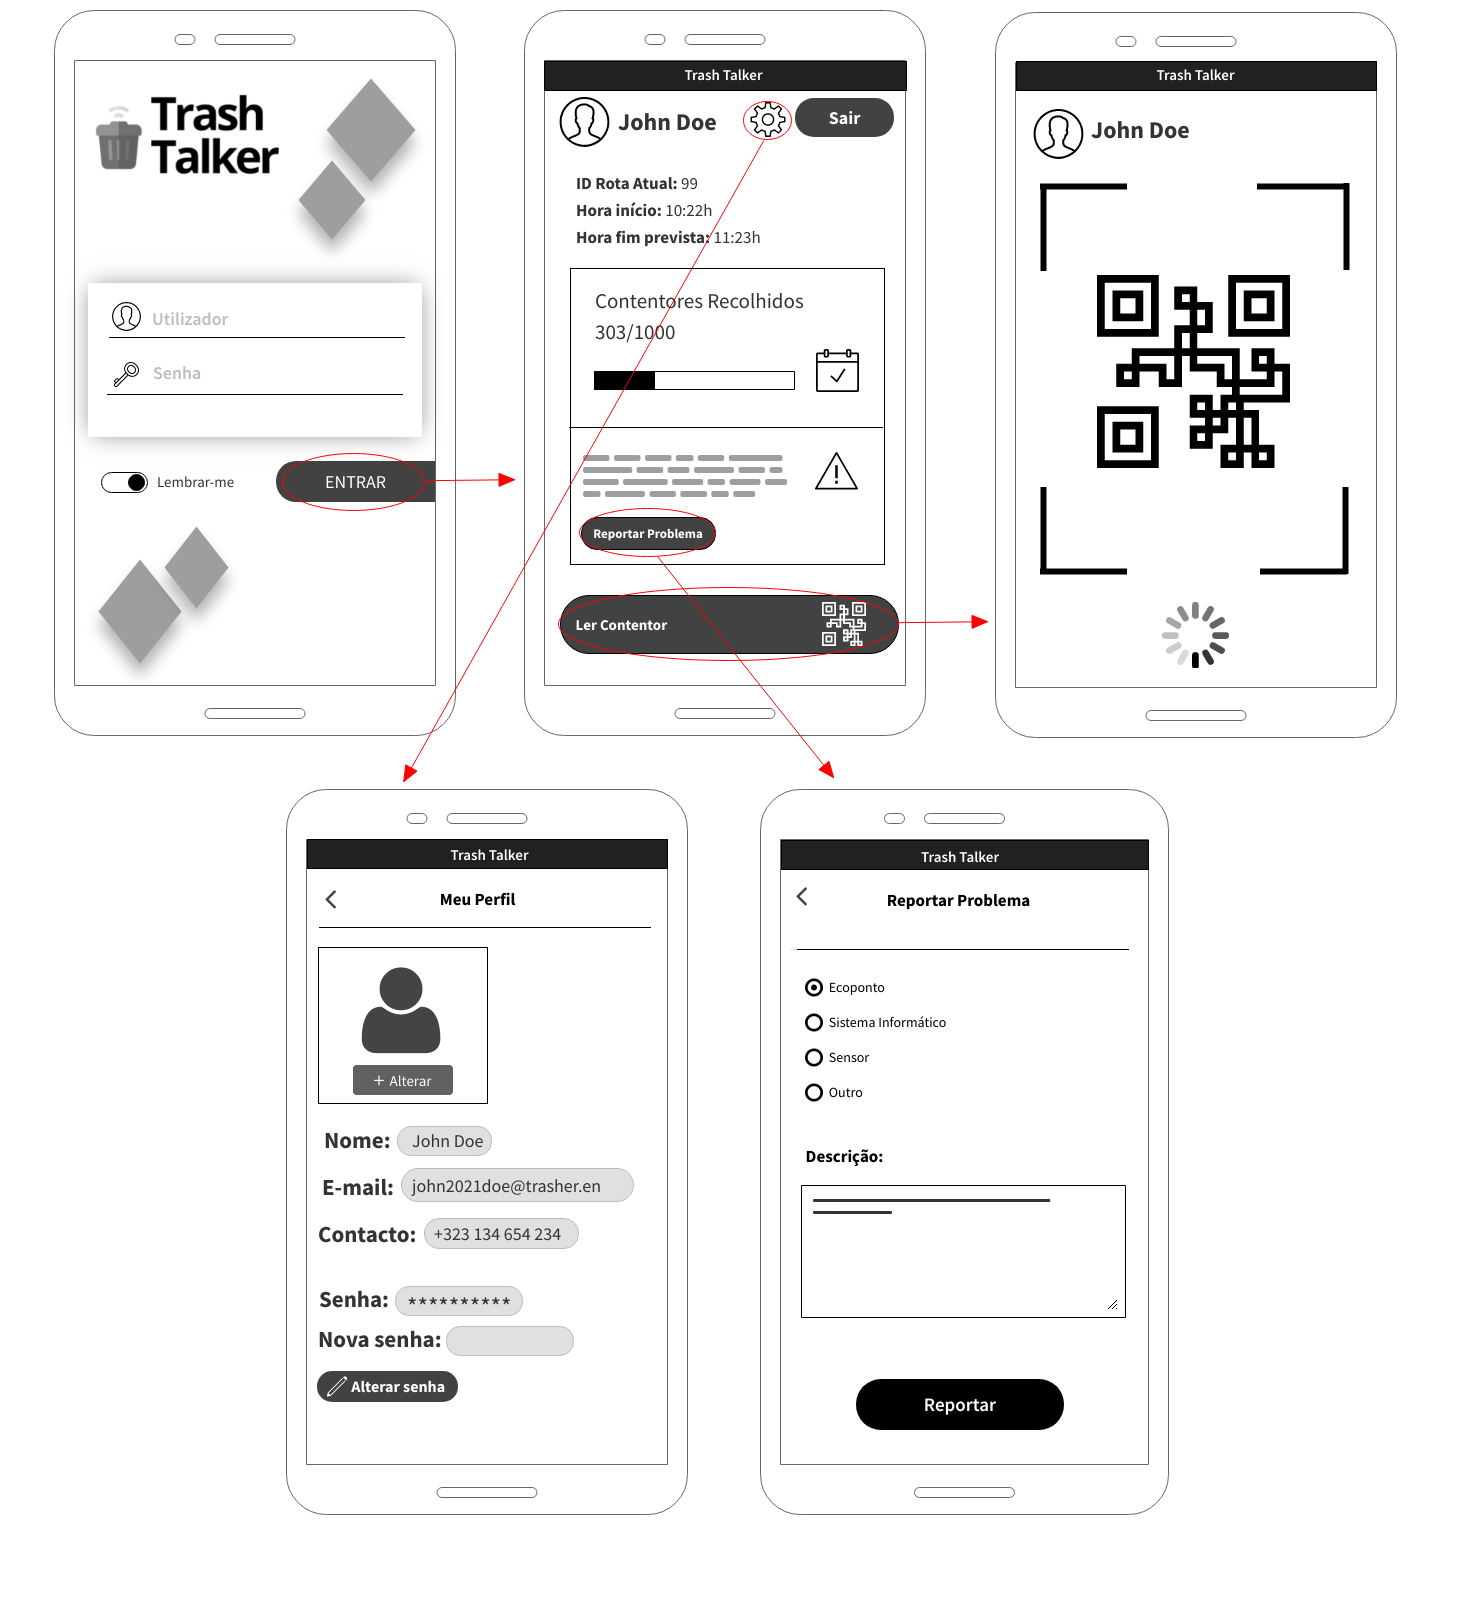
\includegraphics[scale=.30]{imagens/MockupMobile}
		\par \textbf{Mobile Mockup}
		\label{fig:MobileMockup}
	\end{figure}
	
	
	{\let\clearpage\relax \chapter{Use Cases}}
	
	\section{Gerir Contentores}
	
	
	\subsection{Descrição e Prioridade}
	
	Este \textit{use case} tem como objetivo permitir a gestão dos contentores, isto é, integrar no sistema toda a informação do contentor. Na criação do ecoponto é possível atribuir um QR Code a cada contentor e configurar a quantidade de contentores associados (Máximo de 4), tal como o seu tipo e medidas. Será possível também alterar os respetivos dados, ou eliminar o contentor.
	
	\textbf{Cargo: }Gestor  \newline
	\textbf{Prioridade: }Média \newline
	
	\subsection{Sequência de Atividades}
	
	\begin{itemize}
		\item Autenticar no sistema;
		\item Selecionar no menu lateral (Ecopontos);
		\item Clicar no botão criar ecoponto;
		\item Preencher a informação do ecoponto;
		\item Selecionar os contentores com a respetivo tipo e medidas.
	\end{itemize}
	
	
	\subsection{Requisitos Funcionais}
	\textbf{REQ-1:} Atualizar dados do contentor;\newline
	    \textit{- Esta funcionalidade permite ao Gestor Editar o tipo de residuo do contentor.}\newline
	\textbf{REQ-2:} Desativar contentor do ecoponto;\newline
	    \textit{- O Contentor tem um estado associado, ativo ou inativo, esta funcionalidade atrbui o estado inativo ao Contentor.}\newline
	\textbf{REQ-3:} Visualizar detalhes dos contentores;\newline
	\textit{- Permite visualizar os contentores de duas formas; 1-visualizar contentor ataves do id, 2-visualizar todos os contentores.}
	
	\section{Gerir Ecopontos}
	
	\subsection{Descrição e Prioridade}
	Este \textit{use case} permite ao gestor criar ecopontos, visualizar a sua informação, editar os dados e desativar.
	
	\textbf{Cargo: }Gestor  \newline
	\textbf{Prioridade: }Média \newline
	
	\subsection{Sequência de Atividades}
	
	\begin{itemize}
		\item Autenticar no sistema;
		\item Selecionar no menu lateral (Ecopontos);
	\end{itemize}
	
	\subsection{Requisitos Funcionais}
	\textbf{REQ-4: Criar ecoponto};\newline
	\textit{- Permite criar o ecoponto com a seguinte informação: Longitude, Latitude, rua, cidade, codigo-postal e Pais.}\newline\newline

		\underline{Modo de Implementação: }Para criar um ecoponto, deverá fazer-se uso da API GeoLocation que permite a conversão do código postal em latitude e longitude válidas para assegurar o bom funcionamento das rotas automáticas e manuais e visualização no mapa. Esta funcionalidade está disponivel no website, na secção Ecopontos.\newline\newline
		
		\underline{Regras de Negócio: } 
		\begin{itemize}
		\item No momento de criação de um ecoponto, são criados automaticamente 4 contentores(Papel, Plástico,Vidro e Indiferenciado) associados a esse ecoponto.
    	\item Todos os contentores têm dimensões estáticas.
    	\end{itemize}
    	
		\begin{tabular}{|p{5.2in}|p{0.7in}|} \hline 
		\underline{Critérios de Aceitação} \\ \hline 
		Apenas utilizadores com papel de "Manager" podem executar esta funcionalidade \\ \hline 
		Disponibilizar ao cliente formulário de preechimento com morada detalhada no momento de criação do ecoponto.\\ \hline
		Na eventualidade de ocorrência de erros no preenchimento do formulário ou problema na criação do ecoponto, disponibilizar ao cliente o motivo da operação ter falhado.\\ \hline
	\end{tabular}\newline\newline
	

	\textbf{REQ-5: Atualizar dados do ecoponto};\newline
	\textit{- Permite modificar os dados Longitude, Latitude, rua, cidade, codigo-postal e Pais, uma vez que é possivel mudar o ecoponto de lugar.}\newline\newline
	
	\textbf{REQ-6: Desativar ecoponto};\newline
		\textit{- O Ecoponto tem um estado associado, ativo ou inativo, esta funcionalidade atribui o estado inativo ao Ecoponto.}\newline\newline
		
	\textbf{REQ-7: Visualizar detalhes dos ecopontos};\newline
	    \textit{- Permite visualizar os Ecopontos de três formas: 1-visualizar ecoponto pelo id, 2-visualizar todos os Ecopontos, 3-visualizar apenas os Ecopontos Ativos.}\newline\newline
		
		\underline{Modo de Implementação: }Para mostrar a informação de ecopontos são listados todos os ecopontos e depois de cada ecoponto selecionado é possivel ver em detalhe todas as informações do ecoponto. Também é disponibilizado o nivel de ocupação de cada um dos seus 4 contentores atualmente através de um gráfico para facilitar a leitura dos dados. \newline\newline
				
		\underline{Regras de Negócio: } 
		\begin{itemize}
		\item Todos os ecopontos são disponibilizados para consulta de informação mesmo se já tenham sido previamente desativados e não estejam atualmente em funcionamento.
    	\end{itemize}
		
		\begin{tabular}{|p{5.2in}|p{0.7in}|} \hline 
		\underline{Critérios de Aceitação} \\ \hline 
		Apenas utilizadores com papel de "Manager" podem executar esta funcionalidade. \\ \hline 
		Gráfico para visualizar de forma mais intuitiva o grau de ocupação dos contentores.\\ \hline
	\end{tabular}\newline\newline
	
	\section{Gerir Funcionários}
	
	\subsection{Descrição e Prioridade}
	
	Este \textit{use case} permite criar perfis de colaboradores, atualizar os dados e desativar as contas dos mesmos.
	
	\textbf{Cargo: }Gestor  \newline
	\textbf{Prioridade: }Alta \newline
	
	\subsection{Sequência de Atividades}
	
	\begin{itemize}
		\item Autenticar no sistema;
		\item Selecionar no menu lateral (Funcionários);
	\end{itemize}
	
	\subsection{Requisitos Funcionais}
	\textbf{REQ-8: Registar um novo funcionário};\newline
	    \textit{- Existem dois tipos de Funcionarios: O Gestor e o Funcionário que desempenham diferentes papeis na organização e por isso têm diferentes permissões dentro do sistema.} \newline\newline
		
		\underline{Regras de Negócio: } 
		\begin{itemize}
		\item O gestor apenas tem acesso ao website que é voltado para a gestão de todo o processo de recolhas e análise de dados que vão surgindo no dia a dia.
		\item O funcionário, que executam as recolhas, tem acesso à aplicação mobile que permitirá dar inicio e fim das rotas de cada funcionário e efetuar cada recolha em cada contentor.
		\item Apenas é possivel registar um funcionário no website, a aplicação mobile não disponibiliza este tipo de funcionalidade.
		\item Um utilizador do tipo manager pode registar um utilizador do tipo employee, no entanto, não poderá efetuar um registo de outro manager.Apenas uma conta do tipo "Admin" pode fazê-lo.
    	\end{itemize}
		
		\begin{tabular}{|p{5.2in}|p{0.7in}|} \hline 
		\underline{Critérios de Aceitação} \\ \hline 
		Apenas utilizadores com papel de "Manager" podem registar utilizadores do tipo "Employee". \\ \hline 
		Os utilizadores do tipo "Manager não podem registar utilizadores do tipo "Manager".\\ \hline
		Na eventualidade de ocorrência de erros no preenchimento do formulário ou problema no registo de um novo funcionário, disponibilizar ao cliente uma mensagem com o motivo da operação ter falhado.\\ \hline
	\end{tabular}\newline\newline
	
	\textbf{REQ-9: Editar dados de funcionário}\newline
	    \textit{- Esta funcionalidade é da responsabilidade do gestor, permitindo assim editar os dados de um funcionario: Password, Primeiro Nome, ultimo Nome, Email, genero, Rua, Cidade, Codigo-Postal, Pais.}\newline\newline
	    
	\textbf{REQ-10: Desativar funcionário};\newline
	    \textit{- Esta funcionalidade é da responsabilidade do gestor, permitindo assim desativar um funcionario, continuando presente no sistema mas no estado inativo.}\newline\newline
		
		\underline{Regras de Negócio: } 
		\begin{itemize}
		\item Um funcionário depois de desativado não poderá mais ser atribuido a uma rota.
		\item Um funcionário depois de desativado fica impossibilitado de fazer log in na aplicação mobile.
    	\end{itemize}
		
		\textbf{REQ-10: Visualizar dados de funcionário}\newline
	    \textit{- Permite visualizar a lista de todos os funcionários em detalhe.}\newline\newline
		
		\underline{Regras de Negócio: } 
		\begin{itemize}
		\item Esta informação apenas pode ser consultada pelos utilizadores com perfil de "Manager".
    	\end{itemize}
		
	    	\begin{tabular}{|p{5.2in}|p{0.7in}|} \hline 
		\underline{Critérios de Aceitação} \\ \hline 
		Apenas utilizadores com papel de "Manager" podem aceder a esta funcionalidade \\ \hline 
		Credenciais de acesso ao sistema de cada funcionário devem ser ocultadas.\\ \hline
	\end{tabular}\newline\newline
	
	\section{Obter dados estatisticos das recolhas}
	
	\subsection{Descrição e Prioridade}
	
	Este \textit{use case} permite ao gestor obter todos os dados estatísticos das recolhas efetuadas. Esses dados podem ser filtrados por data(s) ou por rota.
	
	\textbf{Cargo: }Gestor  \newline
	\textbf{Prioridade: }Baixa \newline
	
	\subsection{Sequência de Atividades}
	
	\begin{itemize}
		\item Autenticar no sistema;
		\item Selecionar no menu lateral (Dashboard);
	\end{itemize}
	
	\subsection{Requisitos Funcionais}
	\textbf{REQ-12: Consultar dados estatísticos};\newline
	    \textit{- Esta funcionalidade permite ao Gestor consultar informação referente aos dados estatisticos das recolhas.}\newline\newline
		\underline{Modo de Implementação: }Os dados são mostrados em grande parte com recurso a gráficos para facilitar a interpretação da informação da base de dados.Foi utilizado a API do Google Charts para a framework Angular para fazer uso dos gráficos. Esta funcionalidade apenas é disponibilizada no website.
		\newline\newline
		
		\underline{Regras de Negócio: } 
		\begin{itemize}
		\item Um utilizador depois de desativado não poderá mais ser atribuido a uma rota e desabilita a possibilidade de log in na aplicação mobile.
    	\end{itemize}
		
		\begin{tabular}{|p{5.8in}|p{0.7in}|} \hline 
		\underline{Critérios de Aceitação} \\ \hline 
		Apenas utilizadores com papel de "Manager" podem executar esta funcionalidade. \\ \hline 
		Uso de gráficos para apresentação dos dados estatisticos.\\ \hline	
		Uso de filtros de data e local para apresentação dos dados.\\ \hline
		O utilizador deve ser capaz de consultar o número de contentores acima de 90 por cento da sua capacidade\\ \hline
		O utilizador deve ser capaz de consultar o volume de residuos recolhidos de acordo com a data e local selecionados\\ \hline
		O utilizador deve ser capaz de consultar o total de rotas planeadas\\ \hline
		O utilizador deve ser capaz de consultar o volume de cada tipo de residuo de acordo com a data e local selecionados\\ \hline
		O utilizador deve ser capaz de consultar a percentagem de recolha de cada tipo de residuo desde sempre \\ \hline
		O utilizador deve ser capaz de consultar o total de rotas planeadas,canceladas,terminadas e a decorrer desde sempre\\ \hline
		O utilizador deve ser capaz de consultar a taxa de crescimento medio por dia por tipo de residuo a decorrer desde sempre\\ \hline
		O utilizador deve ser capaz de consultar a percentagem de recolha de cada tipo de residuo de um determinado mes desde sempre\\ \hline	
	\end{tabular}\newline\newline
	
	\section{Planear Rota}
	
	\subsection{Descrição e Prioridade}
	
	Este \textit{use case} permite planear uma nova rota. Esta rota é planeada pelo utilizador com o papel de gestor. Aqui poderá optar por planeá-la de forma manual ou automatica. Depois de criada uma rota, esta ficará disponivel tanto no website bem como na aplicação mobile.
	
	\textbf{Cargo: }Gestor  \newline
	\textbf{Prioridade: }Alta \newline
	
	\subsection{Sequência de Atividades}
	
	\begin{itemize}
		\item Autenticar no sistema;
		\item Selecionar no menu lateral (Rotas);
		\item Clicar no botão (Planear Rota);
		\item Escolher entre automático ou manual;
		\item Se manual, preencher dados da rota ;
		\item Clicar no botão (Gerar Rota).
		\item Se automática, preencher dados da rota ;
		\item Clicar no botão (Gerar Rota Automática).
	\end{itemize}
	
	\subsection{Requisitos Funcionais}
	\textbf{REQ-13: Planear rota manual};\newline
	     \textit{- Esta funcionalidade permite ao Gestor planear uma rota de forma manual, definindo o funcionário responsável, a data de inicio, o conjunto de ecopontos que irão ser recolhidos e ordem pela qual irá decorrer.} \newline\newline
		\underline{Modo de Implementação: }Disponibilizar um formulário com todos os ecopontos disponiveis para serem adicionados à recolha. Utilizar a API Distance Matrix para o cálculo das distâncias e a duração entre ecopontos tendo como a referência a sua latitude e longitude. \newline\newline
		
		\underline{Regras de Negócio: } 
		\begin{itemize}
		\item Apenas ecopontos com estado de ativo podem ser apresentados ao utilizador.
		\item Não podem ser criadas rotas com data de inicio anterior à data atual.
	    \item  Esta funcionalidade apenas é disponibilizada no website.
	    \item Apenas se podem associar como funcionário responsável da rota manual utilizadores com perfil de "Employee". 
	\end{itemize}
	
		\begin{tabular}{|p{5.8in}|p{0.7in}|} \hline 
		\underline{Critérios de Aceitação} \\ \hline 
		Disponibilizar apenas ao "Manager" utilizadores registados do tipo "Employee" para potenciais funcionários responsáveis da rota.\\ \hline
		Qualquer erro na submissão da rota deve ser reportado ao cliente o motivo pela qual não foi possivel submeter a rota.\\ \hline
		Disponibilizar ao cliente a data prevista de ocupação total de cada ecoponto, tendo por base o seu histórico de recolhas, para orientar o cliente para a melhor rota possivel. \\ \hline
	\end{tabular}\newline\newline
	
	\textbf{REQ-14: Planear rota automaticamente};\newline
	\textit{- Para planear uma rota de forma automática é necessário especificar o nivel mínimo de ocupação de um ecoponto para este ser introduzido na nova rota a gerar.}
	 \newline\newline
		\underline{Modo de Implementação: }Para a geração de uma rota automática, foi desenhado um algoritmo que tem em conta diferentes variáveis com diferentes pesos. A rota tem inicio num ponto de partida definido, a empresa de recolha. Depois a escolha do ecoponto seguinte é definida pelo ecoponto mais próximo ao ecoponto anterior (recorrendo à API Distance Matrix) mas apenas é adicionado se tem a sua capacidade acima de 80 por cento e se a duração total da rota ao inclui-lo não excede as 7 horas. A capacidade acima de 80 por cento não é contabilizada a percentagem de ocupação atual mas a percentagem de ocupação prevista para o inicio da rota. Estes fatores são executados de forma iterativa até que a condição de paragem for alcançada (7 horas de duração) ou não existirem mais ecopontos que cumpram estes requisitos anteriores. Esta funcionalidade apenas é disponibilizada no website.\newline\newline
		
		\underline{Regras de Negócio: } 
		\begin{itemize}
		\item Apenas ecopontos com estado de ativo podem ser utilizados no algoritmo de construção da rota.
		\item Não podem ser criadas rotas com data de inicio anterior à data atual.
	    \item  Esta funcionalidade apenas é disponibilizada no website.
	    \item Apenas se podem associar como funcionário responsável da rota manual utilizadores com perfil de "Employee". 
	\end{itemize}
	
		\begin{tabular}{|p{5.8in}|p{0.7in}|} \hline 
		\underline{Critérios de Aceitação} \\ \hline 
		Disponibilizar apenas ao "Manager" utilizadores registados do tipo "Employee" para potenciais funcionários responsáveis da rota.\\ \hline
		Qualquer erro na geração da rota deve ser reportado ao cliente o motivo pela qual não foi possivel submeter a rota.\\ \hline
		Disponibilizar ao cliente a duração e distância prevista da rota gerada. \\ \hline
		Mostrar a rota gerada desenhada num mapa no fim da geração da rota. \\ \hline
	\end{tabular}\newline\newline
	
		\textbf{REQ-15: Visualizar rotas registadas};\newline
	\textit{- Este requisito permite ao cliente ver os dados das rotas registadas até ao momento no sistema.}
	 \newline\newline
		\underline{Modo de Implementação: }Esta funcionalidade faz uso da API Google Maps para disponibilizar ao cliente uma mapa com cada rota.  \newline\newline
		
		\underline{Regras de Negócio: } 
		\begin{itemize}
		\item As rotas são apresentadas ao cliente organizadas pelo seu estado.
		\item Os estados possiveis para a rota são Planeada,A Decorrer,Cancelada e Finalizada.
	    \item  Esta funcionalidade apenas é disponibilizada no website..
	\end{itemize}
	
		\begin{tabular}{|p{5.8in}|p{0.7in}|} \hline 
		\underline{Critérios de Aceitação} \\ \hline 
		O circuito da rota deve ser apresentada no mapa.\\ \hline
		As rotas deve ser organizadas e apresentadas tendo em conta os eu estado atual.\\ \hline
	\end{tabular}\newline\newline
	
	\section{Recolha de Ecoponto}
	\subsection{Descrição e Prioridade}
	Este \textit{use case} permite a um funcionário registar a recolha de um contentor através da leitura de um QR-Code existente no contentor. 
	 \newline
			
	\textbf{Cargo: }Funcionário  \newline
	\textbf{Prioridade: }Alta \newline
	\subsection{Sequência de Atividades}
		\begin{itemize}
		\item Autenticar no aplicação mobile;
		\item Aceder Secção Rotas Planeadas;
		\item Iniciar Rota;
		\item Ler QR Code;

	\end{itemize}
	
	\subsection{Requisitos Funcionais}
	\textbf{REQ-16: Iniciar Rota};\newline
	\textbf{REQ-17: Registar Recolha do Contentor};\newline
	\textbf{REQ-18: Finalizar Rota};\newline
	
	\textbf{REQ-16: Iniciar Rota};\newline
	\textit{- Este requisito permite ao cliente dar inicio a uma rota para posteriormente realizar recolhas aos ecopontos.}
	 \newline\newline
		\underline{Regras de Negócio: }
		\begin{itemize}
		\item Apenas é possivel dar inicio a uma rota que tenha o estado de Planeada.
		\item Não é possivel dar inicio a uma rota planeada se já existir outra a decorrer.
	\end{itemize}
	
	\begin{tabular}{|p{5.8in}|p{0.7in}|} \hline 
	\underline{Critérios de Aceitação} \\ \hline 
	Quando o utilizador dá inicio da rota planeada, esta rota é retirada da secção de rotas planeadas e colocada na secção Home como rota a decorrer.\\ \hline
	Apenas devem ser disponibilizas ao utilizador as rotas atribuidas a ele mesmo.\\ \hline
	\end{tabular}\newline\newline
	
	\textbf{REQ-17: Registar Recolha do Contentor};\newline
	\textit{- Este requisito permite ao cliente registar a recolha de um contentor.}
	 \newline\newline
	\underline{Modo de Implementação: }Esta funcionalidade apenas está presente na aplicação mobile. A recolha é registada com a leitura do qr code presente no local.A leitura do QR Code faz uso de uma biblioteca de terceiros - QRCoder v.1.4.3.  \newline\newline
	\underline{Regras de Negócio: }
		\begin{itemize}
		\item Para ser possivel efetuar uma recolha o funcionário terá de ter uma rota a decorrer.
		\item Apenas o funcionário atribuido à rota poderá efetuar este registo.
	    \item Apenas contentores de ecopontos inseridos na rota a decorrer poderão ser registados.
		\item A leitura do QR Code apenas pode ser efetuada antes do descarregamento dos residuos do contentor, para permitir o registo correto do volume de residuos recolhidos.
	\end{itemize}
	
	\begin{tabular}{|p{5.8in}|p{0.7in}|} \hline 
	\underline{Critérios de Aceitação} \\ \hline 
	O utilizador é capaz registar o contentor abrindo a secção de scan do qr code. \\ \hline
	Apenas é possivel abrir o scan do QRCode quando uma rota está a decorrer.\\ \hline
	\end{tabular}\newline\newline
	
		
	\textbf{REQ-18: Terminar Rota};\newline
	\textit{- Este requisito permite ao cliente dar por terminada uma rota iniciada por ele.}
	 \newline\newline
	\underline{Modo de Implementação: }Esta funcionalidade apenas está presente na aplicação mobile. É disponibilizada apenas no momento em que o funcionário tem uma rota em progresso.  \newline\newline
	\underline{Regras de Negócio: }
		\begin{itemize}
		\item Para ser possivel terminar uma rota o funcionário terá de ter uma rota a decorrer.
		\item No minimo é necessário efetuar uma recolha de um contentor para ser possivel terminar a rota.
	\end{itemize}
	
	\begin{tabular}{|p{5.8in}|p{0.7in}|} \hline 
	\underline{Critérios de Aceitação} \\ \hline 
	O utilizador quando termina a rota, a rota desaparece da secção Home e dá indicação de que não há rota a decorrer. \\ \hline
	O utilizador quando termina a rota, a rota aprece na secção de rotas finalizadas..\\ \hline
	\end{tabular}\newline\newline
	
	\section{Reportar problemas}
	
	\subsection{Descrição e Prioridade}
	
	Este \textit{use case} permite ao funcionário reportar problemas sobre os ecopontos, sistemas informáticos, sensores ou outro. Antes da submissão do report é pedida uma breve descrição sobre o problema encontrado.
	
	\textbf{Cargo: }Funcionário  \newline
	\textbf{Prioridade: }Média \newline
	
	\subsection{Sequência de Atividades}
	
	\begin{itemize}
		\item Autenticar no aplicação mobile;
		\item Reportar um problema;
	\end{itemize}
	
	\subsection{Requisitos Funcionais}
	\textbf{REQ-19: Reportar problema}\newline\newline
	    \textit{- Esta funcionalidade tem como objetivo reportar um problema à equipa de gestão da empresa. }\newline
	    
	 \underline{Modo de Implementação: }Esta funcionalidade apenas está presente na aplicação mobile. Não há qualquer tipo de restrição na submissão de problemas, podem ser submetidos em qualqer momento ou estado da rota. O objetivo é manter ao máximo informado a equipa de gestão da empresa. \newline
	
	\underline{Regras de Negócio: }
		\begin{itemize}
		\item É necessário indicar o tipo de problema e a descrição do problema.
		\item As categorias de problemas disponiveis são contentor, sensor, sistema informático e outro.
	\end{itemize}
	
	\begin{tabular}{|p{5.8in}|p{0.7in}|} \hline 
	\underline{Critérios de Aceitação} \\ \hline 
	É disponibilizado um formulário com as opções das categorias do problema. \\ \hline
	Não é possivel submeter um problema sem antes preencher todos os campos do formulário\\ \hline
	\end{tabular}\newline\newline
	
	\section{Autenticar na plataforma}
	
	\subsection{Descrição e Prioridade}
	
	Este \textit{use case} permite ao gestor ou funcionário efetuar login na respetiva plataforma.
	
	\textbf{Cargo: }Gestor, Funcionário  \newline
	\textbf{Prioridade: }Alta \newline
	
	\subsection{Sequência de Atividades}
	
	\begin{itemize}
		\item Autenticar;
	\end{itemize}
	
	\subsection{Requisitos Funcionais}
	\textbf{REQ-20: Autenticar no sistema};\newline
	    \textit{- Para se autenticar na aplicação mobile o utilizador tera de estar registado, esta funcionalidade passa pelo gestor que tem a tarefa de registar os funcionários, para aceder a aplicação os funcionarios precisam introduzir o nome de utilizador e password, que lhe foram atribuidas pelo Gestor.}\newline\newline
	    
    	 \underline{Modo de Implementação: }Aqui a implementação divide-se em dois ambientes distintos. A aplicação mobile disponibiliza a autenticação através do username e password apenas para utilizadores do tipo Funcionario, já no website a autenticação efetua-se tendo por base o username e password mas apenas para utilizadores com perfil de gestor.\newline
	
    	\underline{Regras de Negócio: }
    		\begin{itemize}
    		\item  Apenas utilizadores registados no sistema podem aceder tanto à aplicação mobile bem como o website, não havendo qualquer tipo de disponibilização de informação interna da organização a utilizadores visitantes anónimos.
    		\item A password é encriptada antes de guardar na base de dados para salvaguardar a sua confidencialidade e segurança.
    	\end{itemize}
	
    	\begin{tabular}{|p{5.8in}|p{0.7in}|} \hline 
    	\underline{Critérios de Aceitação} \\ \hline 
    	Se o username e password não forem aceites pelo servidor é mostrado ao utilizador uma mensagem de alerta. \\ \hline
    	\end{tabular}\newline\newline

	
	{\let\clearpage\relax \chapter{Other Nonfunctional Requirements}}
	
	\section{Requisitos de Performance}
	\begin{itemize}
		\item A base de dados deve estar normalizada para reduzir a redundância e melhorar a performance.
	\end{itemize}
	
	
	\section{Security Requirements}
	\begin{itemize}
		\item Necessário ter uma conta registada no sistema para ter acesso a aplicação.
		\item Autenticação de utilizadores via JWT.
	\end{itemize}

	{\let\clearpage\relax \chapter{Diagramas}}
		\section{Diagrama de Classes}

	\begin{figure}[H]
		\centering
		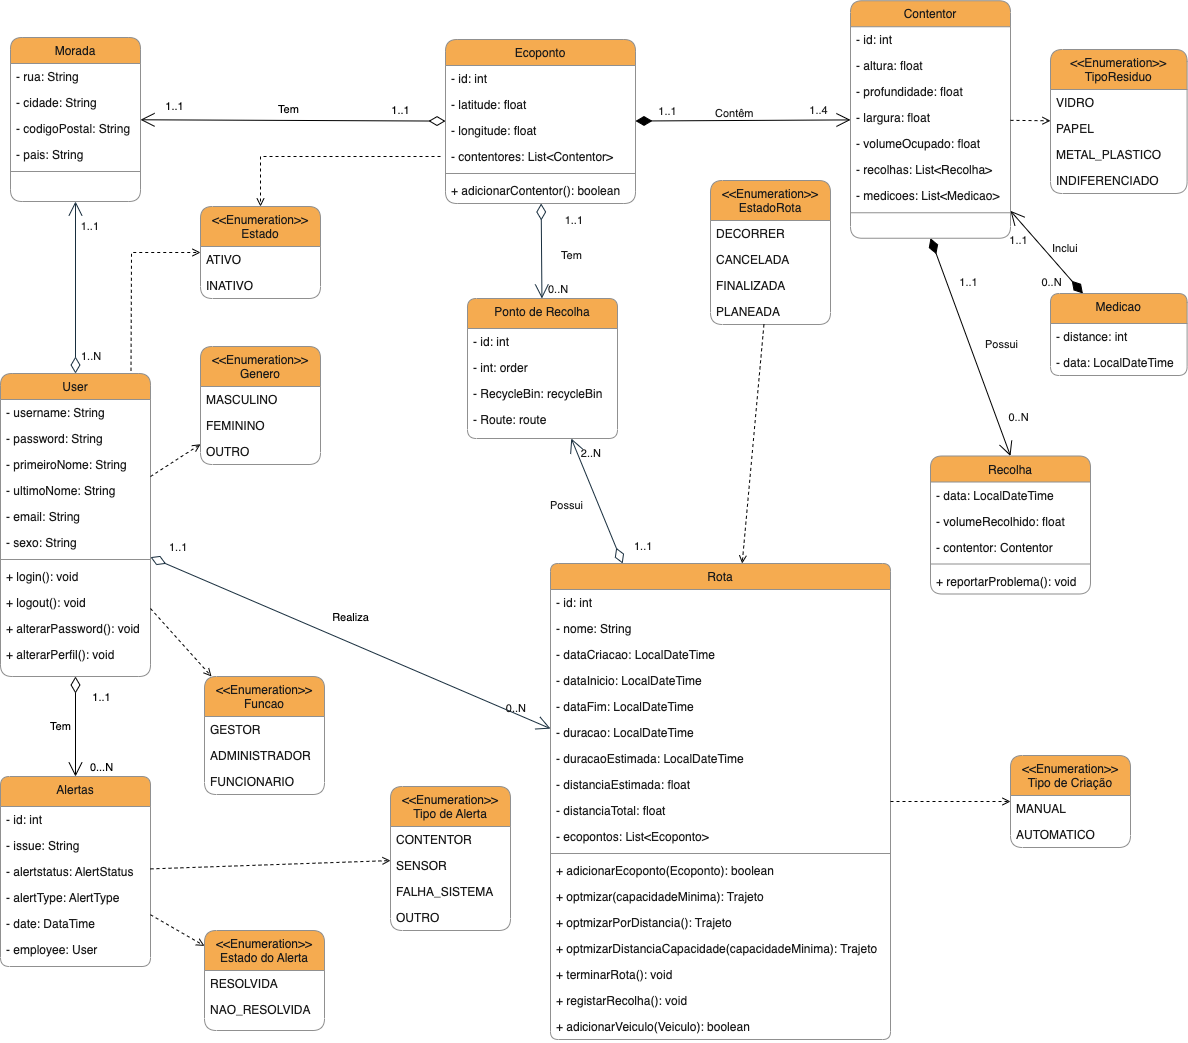
\includegraphics[scale=.4]{imagens/class_Diagram.png}
		\par \textbf{Diagrama de Classes}
		\label{fig:classDiagram}
	\end{figure}

\end{document}